\chapter{Architektura Kodu i Implementacja}

W niniejszym rozdziale przedstawiono strukturę implementacji systemu oraz omówiono kluczowe fragmenty kodu źródłowego odpowiedzialne za realizację założeń projektowych.

\section{Klasy i mechanizm hermetyzacji}
Na poniższym zrzucie ekranu (Rys. 2.1) przedstawiono implementację struktury klas zorientowanej obiektowo. Klasa bazowa \texttt{Produkt} definiuje uniwersalne właściwości obiektów, natomiast za pomocą dekoratorów \texttt{@property} oraz \texttt{@cena.setter} zrealizowano hermetyzację i automatyczną walidację poprawności ceny. Klasy pochodne \texttt{Elektronika} oraz \texttt{Odziez} dziedziczą po klasie bazowej i nadpisują metodę \texttt{pokaz\_szczegoly()}, implementując paradygmat polimorfizmu.

\begin{figure}[H]
    \centering
    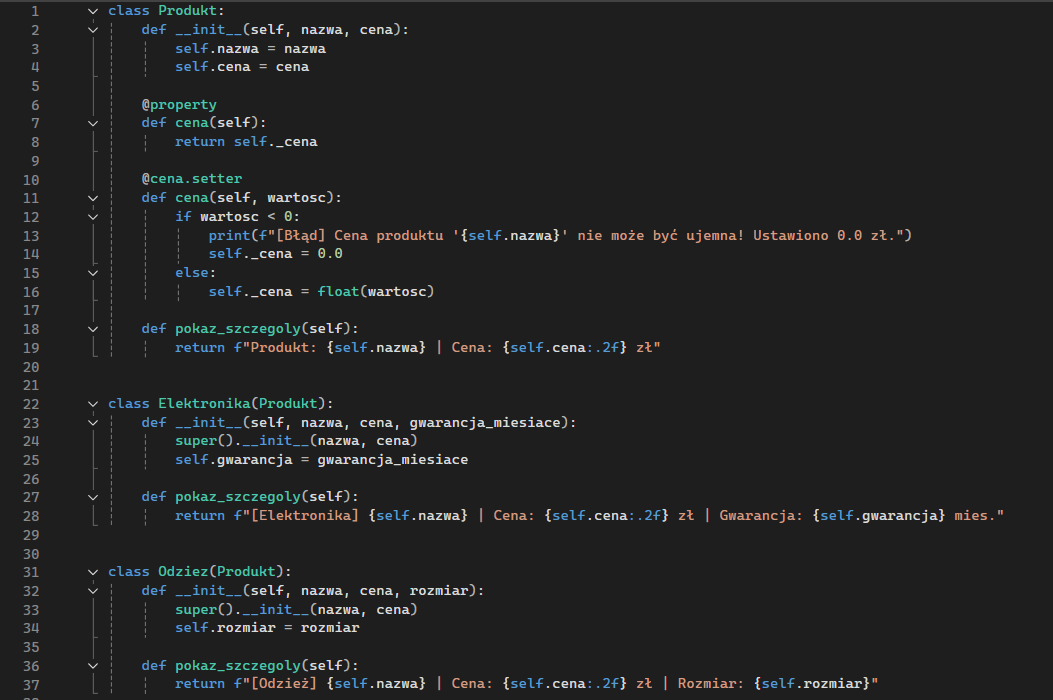
\includegraphics[width=0.9\textwidth]{screen_kod_klasy.png}
    \caption{Implementacja klas bazowych, pochodnych oraz walidacji ceny.}
    \label{fig:kod_klasy}
\end{figure}

\section{Logika biznesowa i listy składane}
Klasa \texttt{Sklep} odpowiada za logikę biznesową systemu oraz zarządzanie kolekcją obiektów przechowywanych w dynamicznej liście \texttt{asortyment} (Rys. 2.2). W metodach filtrujących zastosowano technologię list składanych (\textit{list comprehensions}), która pozwala na wydajne i zwięzłe przeszukiwanie struktur danych w języku Python bez konieczności stosowania wielolinijkowych tradycyjnych pętli.

\begin{figure}[H]
    \centering
    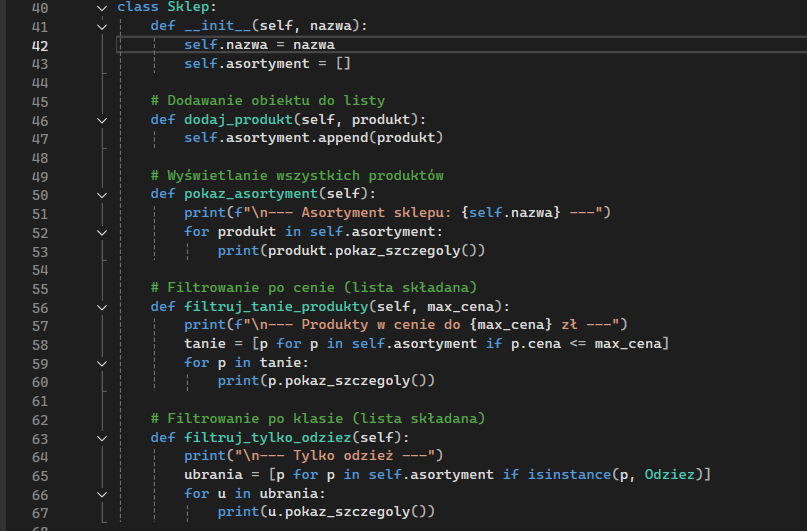
\includegraphics[width=0.9\textwidth]{screen_kod_sklep.png}
    \caption{Klasa zarządzająca asortymentem z użyciem list składanych.}
    \label{fig:kod_sklep}
\end{figure}

\newpage 
\section{Główny punkt wejścia i pętla menu}
Ostatni fragment kodu źródłowego (Rys. 2.3) odpowiada za uruchomienie aplikacji oraz obsługę interakcji z użytkownikiem w czasie rzeczywistym. W bloku \texttt{if \_\_name\_\_ == "\_\_main\_\_"} następuje inicjalizacja obiektu klasy \texttt{Sklep} i zasilenie go startowymi danymi testowymi (w tym produktem o ujemnej cenie w celu przetestowania walidacji). Sterowanie aplikacją zorganizowano przy użyciu nieskończonej pętli \texttt{while True} oraz instrukcji warunkowych \texttt{if-elif-else}, które pobierają wybór użytkownika przez funkcję \texttt{input()} i przekierowują żądania do odpowiednich metod klasy sterującej.

\begin{figure}[H]
    \centering
    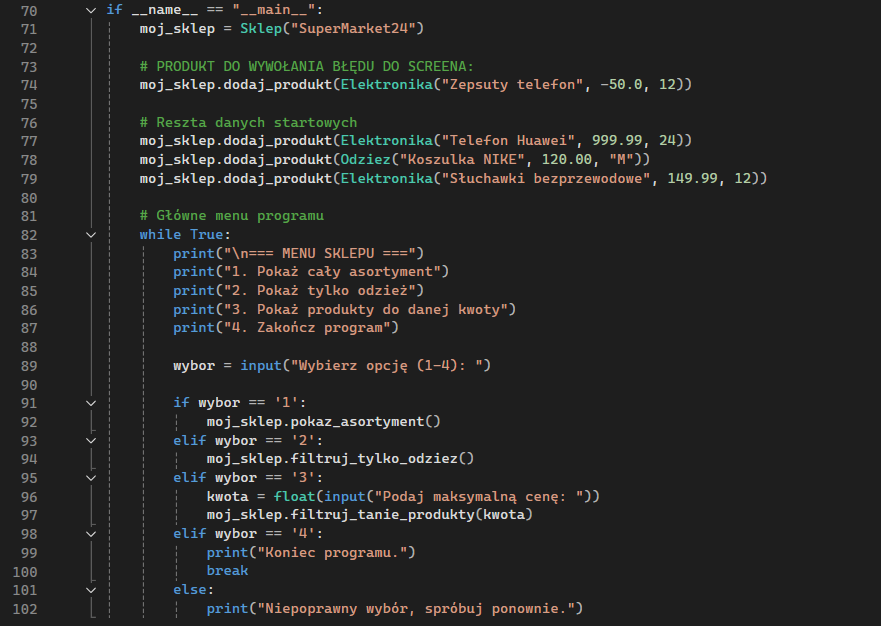
\includegraphics[width=0.9\textwidth]{screen_kod_menu.png}
    \caption{Główny punkt wejścia do programu oraz implementacja pętli menu.}
    \label{fig:kod_menu}
\end{figure}
